\documentclass[
prx
,twocolumn
,nofootinbib
,floatfix
,superscriptaddress
]{revtex4-2} 
%\pdfoutput=1

% \usepackage{mathptmx}
% \DeclareMathAlphabet{\mathcal}{OMS}{cmsy}{m}{n}

\usepackage{notes2bib}
\usepackage{natbib}
\usepackage{gensymb}
\usepackage{amsthm}
\usepackage{amsmath}
\usepackage{color}
\usepackage{bm}
\usepackage{amsmath,amssymb}
\usepackage{amsfonts}
\usepackage{dsfont}
\usepackage{graphicx}
\usepackage{float}
\usepackage{subfigure}
\usepackage{verbatim}
\usepackage{amsfonts}
\usepackage{bbold}
\usepackage{dcolumn}
\usepackage{bm}
\usepackage[dvipsnames]{xcolor}
\usepackage{listings}
\definecolor{blueprl}{RGB}{46,48,146}
\usepackage[pdftex,colorlinks=true,urlcolor=blueprl,citecolor=blueprl,linkcolor=blueprl]{hyperref}
\usepackage{mathrsfs}
%\usepackage{filecontents}
\usepackage{mathtools}
\usepackage{times}
\usepackage{color}
\usepackage[dvipsnames]{xcolor}

\usepackage{braket}
\newtheorem{lemma}{Lemma}
\newtheorem{theorem}{Theorem}
\newtheorem{proposition}{Proposition}
\newenvironment{prooft1}[1][Proof (Theorem 1)]{\noindent\textbf{#1.} }{\ \rule{0.5em}{0.5em}}
\newenvironment{prooft2}[1][Proof (Theorem 2)]{\noindent\textbf{#1.} }{\ \rule{0.5em}{0.5em}}
\def\ketbra#1#2{{\vert#1\rangle\!\langle#2\vert}}
\newcommand{\tr}{\mbox{Tr}}
\newcommand*\mean[1]{\bar{#1}}
\DeclareMathOperator{\sign}{sign}
\DeclareMathOperator{\sinc}{sinc}
\DeclareMathOperator{\arccosh}{arccosh}
\DeclareMathOperator{\rect}{rect}

\newcommand{\cam}[1]{\textcolor{violet}{ #1}}
\usepackage{soul}
\newcommand{\crss}[1]{\textcolor{orange}{\st{ #1}}}
\newcommand{\comn}[1]{\textbf{\textcolor{blue}{AM:#1~}}}

% \usepackage{tgtermes}


\iffalse 
\usepackage{newtxtext,newtxmath}
\fi 

\usepackage{mathtools}
\usepackage{dsfont}
\usepackage[mathscr]{euscript}
\usepackage{amsmath}
\usepackage{graphicx}
\usepackage{dcolumn}
\usepackage{bm}
\usepackage{epsfig}
\usepackage{amssymb,latexsym,mathrsfs}
\usepackage{graphicx}
\usepackage{color}
%\usepackage{epstopdf}
\usepackage{hyperref}
\usepackage{float}
\usepackage{diagbox}
%\usepackage[backend=bibtex,style=phys]{biblatex}
  \usepackage{cancel}
  \usepackage[normalem]{ulem}

%\addbibresource{bibliography.bib}

\definecolor{vividviolet}{rgb}{0.62, 0.0, 1.0}
\definecolor{amaranth}{rgb}{0.9, 0.17, 0.31}
\definecolor{palatinateblue}{rgb}{0.15, 0.23, 0.89}
\definecolor{brightpink}{rgb}{1.0, 0.0, 0.5}
\definecolor{cornflowerblue}{rgb}{0.39, 0.58, 0.93}
\definecolor{deepcarminepink}{rgb}{0.94, 0.19, 0.22}
\definecolor{radicalred}{rgb}{1.0, 0.21, 0.37}
\definecolor{blueblue}{RGB}{21,47,181}
\definecolor{greengreen}{RGB}{65,166,16}
\newcommand{\ranglem}{|0_M\rangle }
 \newcommand{\rbm}[1]{{\color{red}\bf [Robb: #1]}}
\newcommand{\tcb}{\textcolor{blue}}
\newcommand{\tcr}{\textcolor{red}}
\usepackage{xtab,afterpage}
\usepackage{hyperref}
\usepackage{setspace,calc}
 \newcommand{\mz}{\color{green}}

%\hypersetup{
%    colorlinks=true,
%    linkcolor=red,
%    citecolor=blue,
%} 

\hypersetup{ linktoc=all,
    colorlinks, linkcolor={blueblue},
    citecolor={greengreen}, urlcolor={blueblue}
}
\newcommand{\changeurlcolor}[1]{\hypersetup{urlcolor=#1}}
% Making life easier
\newcommand{\be}{\begin{equation}}
\newcommand{\ee}{\end{equation}}
\newcommand{\bs}{\begin{split}} 
\newcommand{\bea}{\begin{eqnarray}}
\newcommand{\eea}{\end{eqnarray}}
\newcommand{\infint}{\int_{-\infty }^{\infty }}
\newcommand{\vt}{\vphantom{\frac{1}{2}}}
\newcommand{\mike}[1]{\textcolor{red}{[{\bf MG}: #1]}} 
\newcommand{\eric}[1]{\textcolor{magenta}{[{\bf EL}: #1]}} 
% useful symbols
\newcommand{\om}{\Omega_m}
\newcommand{\Om}{\Omega_m}
%\newcommand{\ode}{\Omega_{de}}
\newcommand{\ode}{\Omega_{\rm de}}
\newcommand{\oode}{{\mathcal O}(\Omega_{\rm de})}
\newcommand{\op}{\Omega_\phi}
\newcommand{\lcdm}{$\Lambda$CDM} 
\newcommand{\al}{\alpha} 
\newcommand{\kap}{\kappa} 
\newcommand{\kp}{\kappa}
\newcommand{\eps}{\epsilon}
\newcommand{\event}{Even$t^{-1}$} 
\renewcommand{\d}[1]{\ensuremath{\operatorname{d}\!{#1}}}
\def\nn{\nonumber} 
 \newcommand{\jf}[1]{{\color{blue} [JF: #1]}}
 \newcommand{\bluedit}[1]{{\color{blue} #1}}
\newcommand{\non}{\nonumber} 
 \newcommand{\redit}[1]{{\color{red} #1}}
\newcommand{\p}{\partial} 
\newcommand{\D}{\mathrm{d}}
\newsavebox{\myhbar}
\newcommand{\VT}{\vphantom{\frac{1}{2}}}


\begin{document}

\newcommand{\CQCT}{\affiliation{Centre for Quantum Computation \& Communication Technology, School of Mathematics \& Physics, The University of Queensland, St.~Lucia, Queensland, 4072, Australia}}
\newcommand{\FUB}{\affiliation{Dahlem Center for Complex Quantum Systems, Freie Universit\"at Berlin, 14195 Berlin, Germany}}

\title{Relativistically invariant Bohmian trajectories of photons}
\author{Joshua Foo}
\email{joshua.foo@uqconnect.edu.au}
\CQCT

\author{Estelle Asmodelle}
\CQCT

\author{Austin P. Lund}
\FUB
\CQCT

\author{Timothy C. Ralph}
\email{ralph@physics.uq.edu.au}
\CQCT

\begin{abstract}
Bohmian mechanics is a nonlocal hidden-variable interpretation of quantum theory which predicts that particles follow deterministic trajectories in spacetime. Historically, the study of Bohmian trajectories has been restricted to nonrelativistic regimes due to the widely held belief that the theory is incompatible with special relativity. Here we derive expressions for the relativistic velocity and spacetime trajectories of photons in a Michelson-Sagnac-type interferometer. The trajectories satisfy quantum-mechanical continuity and the relativistic velocity addition rule. Our new velocity equation can be operationally defined in terms of weak measurements of momentum and energy. We finally propose a modified Alcubierre metric which could give rise to these trajectories within the paradigm of general relativity. 
\end{abstract}

\date{\today}

\maketitle

Ever since the conception and early development of quantum mechanics there have been debates over how to consistently interpret the mathematical objects it defines. Many of these debates, such as those concerning the physical meaning of the wavefunction \cite{aharanovPhysRevA.47.4616,weinberg_2015,Ringbauer_2015}, continue to this day. The predominant view among present-day physicists is the Copenhagen interpretation, which treats the square of the wavefunction, 
\begin{align}\label{eq1schrodingerdensity}
    \rho_S(x,t) &= | \psi(x,t) |^2,
\end{align}
as the probability of finding a particle at the spacetime point $(x,t)$, a postulate known as the Born rule. Thus, the Copenhagen interpretation is, by its very definition, an intrinsically probabilistic formulation of quantum theory. This indeterminacy is also manifest in the Heisenberg uncertainty principle, which forbids observations that would permit simultaneous knowledge of the precise position and momentum of a particle. 

In contrast with standard interpretations of quantum theory, Bohmian mechanics is a deterministic, nonlocal theory first proposed by de Broglie \cite{debroglie:jpa-00205292} and then formalised by Bohm \cite{bohmPhysRev.85.166,bohm2006undivided}. As described in Bell's famous paper, it is a theory of the nonlocal hidden-variable type \cite{EPRPhysRev.47.777,bellPhysicsPhysiqueFizika.1.195}. Specifically, the wavefunction (itself evolving according to the Schr\"odinger equation) determines the evolution of a nonlocal guiding potential which in turn, governs the dynamics of the particles. Notably, the Bohmian interpretation recovers many of the standard results of nonrelativistic quantum mechanics such as the Born rule, where instead of describing the probability distribution of a particle's location, $\rho(x,t)$ is now interpreted as the density of particle trajectories given some initial distribution.

Bohmian mechanics has been extended and applied to a diverse range of nonrelativistic settings. Early works by Hirschfelder et.\ al.\ \cite{hirschfelderdoi:10.1063/1.1681899}, Philippidis et.\ al.\ \cite{philippidis1979quantum} and Dewdney et.\ al.\ \cite{dewdney1982quantum} focused on the scattering of massive particles off different kinds of potential barriers. Dewdney et.\ al.\ and Durr et.\ al.\ extended the theory to include spin-1/2 particles and provided a description of EPR correlations \cite{dewdney1988spin,durr1996bohmian}; Leavens applied it to the measurement of arrival times \cite{leavensPhysRevA.58.840}, while others have utilised Bohmian mechanics in the context of quantum chaos \cite{durr1992quantum,FRISK1997139}. 

Interest in Bohmian mechanics was reinvigorated following the development of a weak measurement model by Wiseman \cite{Wiseman_2007}, from which an operational definition for the velocity and hence the spacetime trajectory of nonrelativistic particles can be determined. Using this weak measurement based formalism, such trajectories have been observed experimentally by Kocsis et.\ al.\  \cite{kocsis2011observing} and Mahler et.\ al.\ \cite{mahler2016experimental}. The weak measurement approach used by Wiseman allows one to extract the ensemble average of an observable over a large number of trials, while only weakly perturbing the system. In \cite{Wiseman_2007}, an operational definition for the velocity $V(x,t)$ of nonrelativistic particles was made in terms of a weak measurement of position at time $t$, followed by a strong measurement of position (a projection onto a position eigenstate) a short time $\delta t$ later. This definition recovers the usual quantum-mechanical continuity equation, 
\begin{align}\label{2continuity}
    \frac{\p \rho_S(x,t)}{\p t} &= - \frac{\p j_S(x,t) }{\p x} ,
\end{align}
where $j_S(x,t) = V(x,t) \rho_S(x,t)$ is the conserved probability current. One can obtain the velocity explicitly from Eq.\ (\ref{2continuity}):
\begin{align}\label{3velocity}
    V(x,t) &= - \frac{1}{\rho_S(x,t)} \int\D x \: \frac{\p \rho_S(x,t)}{\p t}, 
\end{align}
where the conserved probability current can be identified as $j_S(x,t) = - \int\D x \: \p \rho_S(x,t)/\p t$. 

Despite its successes, a formidable challenge continues to face the proponents of the Bohmian interpretation, namely its apparent conflict with special relativity. To date, the theory has not been extended to relativistic particle trajectories. This apparent incompatibility is typically attributed to the difficulties in constructing a physically meaningful (i.e.\ positive definite) and relativistically invariant four-vector probability current and density \cite{BOHM1987321,Struyve:2004xd}. In his treatment of electromagnetic scattering, Bohm asserted that a particle description of photons is fundamentally inconsistent, insisting that a field description is necessary \cite{BOHM1987321}. In a similar vein, Flack and Hiley have raised concerns that a relativistic treatment of photon trajectories is likely unphysical due to the existence of reference frames in which its velocity is zero \cite{flack_hiley_2015}. Thus, even in recent works using modified theories of relativistic quantum mechanics \cite{Ghose_2001,Jalalzadeh_2019} and classical electrodynamics \cite{Davidovi__2009,SANZ2010763}, a low-energy or massive-particle limit is inevitably taken when analysing particle trajectories. For example, in the context of photon trajectories as measured by Kocsis et.\ al.\ in a double-slit arrangement, it was the slow transverse velocities that were modelled as obeying a nonrelativistic energy dispersion. A consistent theory of Bohmian particle trajectories based on observed velocity fields in relativistic regimes has not been developed. 

In this article we propose a velocity equation describing the Bohmian trajectories of relativistic particles, specifically photons possessing a relativistic energy dispersion. Our new velocity equation can be derived operationally through weak measurements of the particle momentum and energy, which we respectively identify with the Klein-Gordon conserved probability current and density.  We use the Klein-Gordon theory to capture the essential Lorentz relativistic properties of photons whilst understanding that this is a simplification of a full electrodynamical theory. We find that Wiseman's weak measurement definition fails in the relativistic limit due to tacit nonrelativistic assumptions, most notably a privileged timeslice on which measurements of the particle position are made. Our new velocity equation is invariant under Lorentz boosts, equivalently satisfying the relativistic velocity addition rule. Our analysis focuses on the `optical' limit where the distribution of wavevectors is concentrated well away from zero.  This yields a Klein-Gordon probability density which remains positive definite, avoiding the well-known pathologies of the single-particle theory. In the paraxial (massive-particle) limit, our new velocity equation reduces to that predicted by Wiseman's nonrelativistic theory. We finally draw a connection between the relativistic wavefunction and the Alcubierre metric \cite{Alcubierre_1994}, proposing this as a relativistic generalisation to the quantum potential \cite{bohmPhysRev.85.166} which guides the particle in the nonrelativistic limit.

Throughout this article, we utilise natural units, $\hslash = c = 1$ and the metric signature $(-,+,+)$ in (2+1)-dimensional Minkowski spacetime. 


\section{Results}
\subsection{Physical setup}
The physical geometry of our system, represented as a Michelson-Sagnac interferometer, is depicted in Fig.\ \ref{fig:setup} on a background of flat spacetime in (2+1)-dimensions. A controllable beamsplitter diverts the path of the single photon to the top or bottom branch of the interferometer. Of course within a conventional interpretation of quantum mechanics, the photon traverses both arms of the interferometer in superposition, whereas in Bohmian mechanics the photon is guided by the pilot wave along one of the paths. 
\begin{figure}[ht]
    \centering
    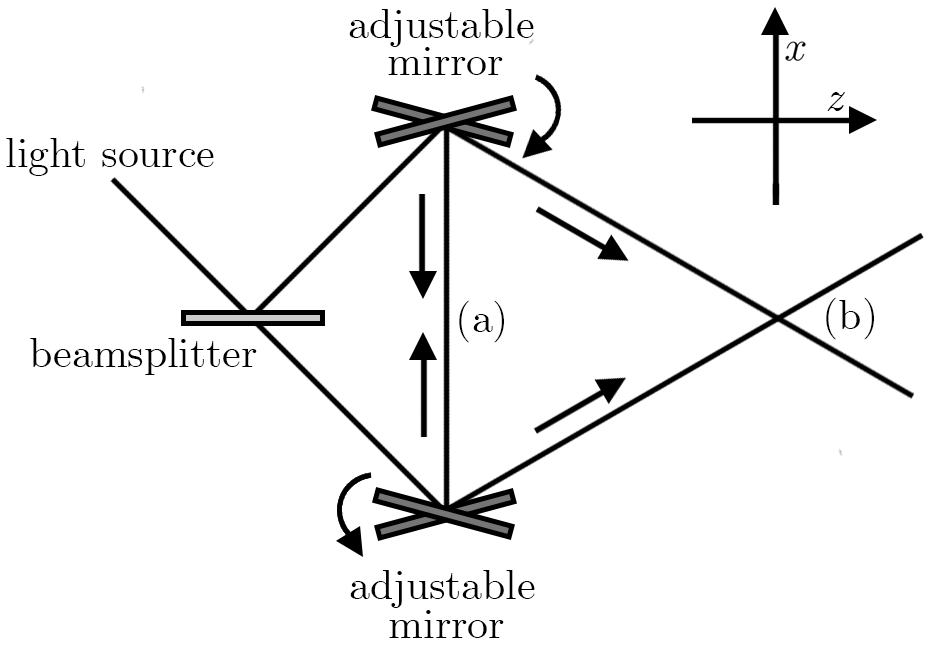
\includegraphics[width=\linewidth]{Fig1schematic.png}
    \caption{Schematic diagram illustrating the geometry of the setup. The adjustable mirrors control the path of the photon in the transverse direction, which can be tuned to produce a head-on collision (a) or a grazing collision (b).}
    \label{fig:setup}
\end{figure}
The adjustable mirrors reflect the photon towards the centre of the apparatus. In scenario (a), the wavevector in the $z$-direction is approximately zero, $k \equiv k_x \gg k_z$, which we refer to as a head-on collision. Scenario (b) depicts the general case in which the photon possesses a non-zero wavevector component in the $z$-direction, which we refer to as the relativistic grazing scenario. When $k_z \gg k$, the $x$-component of the photon velocities are slow; this nonrelativistic regime is known as the paraxial limit. In the literature, only the paraxial limit has been studied in analogous setups.

\subsection{Weak values and weak measurements}
To obtain the relativistic velocity equation, we will begin from an operational starting point, using the notion of weak measurements. Weak measurements were first proposed by Aharonov, Albert, and Vaidman \cite{aharonovPhysRevLett.60.1351} as a method of performing arbitrarily precise measurements of quantum-mechanical observables with minimal system disturbance, where the example of a particle spin was used. To understand this concept, consider a large ensemble of $N$ particles each prepared in the same quantum state. So long as the measurements of the observable $\hat{a}$ of the particles is weak, by performing this measurement many times on each member of the ensemble, the average value of the observable can be extracted with minimal disturbance to each individual particle. While the measurement only weakly perturbs the system, and thus the measurement signal is accompanied by a large amount of noise, the measurement uncertainty scales as $1/\sqrt{N}$ while the average value $\langle \hat{a}\rangle$ remains the same. 

A `weak value' extends this notion of weak measurement by introducing a subsequent strong measurement and performing post-selection on the ensemble based on this strong measurement.
Formally, we can define the weak value, denoted $\prescript{}{\langle \phi|}{\langle \hat{a}_w} \rangle_{|\psi\rangle}$, as the mean value of the observable $\hat{a}$ obtained from many weak measurements on an ensemble of particles each prepared in the state $|\psi\rangle$, postselecting only those particles where a later strong measurement reveals the system to be in the state $|\phi\rangle$. This results in the following definition \cite{aharanovPhysRevA.47.4616}:
\newcommand{\wv}[3]{{}_{#1}\langle {#2}_w \rangle_{#3}}
\begin{align}\label{eqwv4}
    \wv{\bra{\phi}}{\hat{a}}{\ket{\psi(t)}} =
    \text{Re} \frac{\bra{\phi}\hat{a}\ket{\psi(t)}}{\braket{\phi|\psi(t)}}.
\end{align}
Garretson et.\ al.\ have also provided a derivation of Eq.\ (\ref{eqwv4}) in the language of generalised measurements \cite{Garretson_2004}. 

\subsection{The relativistic velocity equation}
In deriving the relativistic velocity equation, we focus our analysis on the particle dynamics in the $x$-direction, in accordance with the setup shown in Fig.\ \ref{fig:setup}. Meanwhile, variables in the $z$-direction are treated as constants of the problem. Let us begin with the most general definition of velocity as a rate of change of the position variable $x$ with respect to time,
\begin{align}\label{eq5velocity}
    V(x,t) &= \frac{\D x}{\D t} = \frac{\D x}{\D \tau} \cdot \frac{\D \tau}{\D t} = \frac{p_x}{E}.
\end{align}
Equation \ref{eq5velocity} is a relativistically invariant quantity; the coordinate time, $t$, and position, $x$, form a relativistic spacetime two-vector $\textbf{x} = (t,x)$, as do the total energy of the photon and the $x$ component of the momentum; $\textbf{p} = (E,p_x)$. Equipped with the toolkit of weak values and in view of this relativistically invariant definition of the velocity, we propose the following definition for the relativistic weak value velocity of single photons:
\begin{align}\label{velocity4}
    V(x,t) &= \frac{\prescript{}{\langle x | }{\langle \hat{k}_w \rangle}_{|\psi(t)\rangle}}{\prescript{}{\langle x |}{\langle \hat{H}_w \rangle }_{|\psi(t)\rangle}} = \frac{\text{Re} \langle x| \hat{k} | \psi(t)\rangle}{\text{Re} \langle x | \hat{H} | \psi(t) \rangle } .
\end{align}
In Eq.\ (\ref{velocity4}), $\hat{k} \equiv \hat{k}_x$ is the momentum operator (modulo a multiplicative factor of $\hslash$ set to unity) while $\hat{H}$ is the Hamiltonian. The weak values of these operators are defined with respect to an initial preparation for the ensemble of particles in the state $|\psi\rangle$ and projected onto the single-particle position eigenstate $|x\rangle$ (i.e.\ postselection at the spacetime point $(x,t)$),
\begin{align}\label{eq7x}
    |x \rangle &= \int\D k \: e^{-ikx } | k \rangle .
\end{align}
Let us return to our new velocity equation. We prepare the particle in the state 
\begin{align}
    |\psi\rangle &= \int\D k \:f(k) |k \rangle 
\end{align}
where $f(k) \equiv f(k_x)$ determines the initial distribution of the particle momenta, and $\hat{a}_k^\dagger | 0 \rangle = |k\rangle \equiv | k_x \rangle$ is a single-particle momentum eigenstate. Using the Klein-Gordon field momentum and Hamiltonian expressions and projecting onto $|x \rangle$, we find that Eq.\ (\ref{velocity4}) reduces to
\begin{align}\label{velocity6}
    V(x,t) &= \frac{2 \text{Im} \: \psi^\star(x,t) \p^x \psi(x,t)}{2 \text{Im} \: \psi^\star(x,t) \p^t  \psi(x,t)}.
\end{align}
where $\psi(x,t) = \langle x |\psi(t)\rangle$ is the time-dependent position-space wavefunction. In Eq.\ (\ref{velocity6}), we readily identify the numerator and denominator of the velocity equation with the conserved probability current and density obtained from the single-particle Klein-Gordon equation:
\begin{align}\label{bohmianvelocity10}
    V(x,t) &= \frac{j_{K}(x,t)}{\rho_{K} (x,t)}. 
\end{align}
Equation \ref{bohmianvelocity10} has the same form as the definition of particle velocity in Bohmian mechanics, Eq.\ (\ref{3velocity}). The crucial difference is the introduction of the Klein-Gordon current and density, which form the components of a spacetime two-vector
\begin{align}
    j_{K}^\mu (x,t) &= 2 \text{Im} \:  \psi^\star(x,t) \p^\mu \psi(x,t) ,
\end{align}
and are by construction relativistically invariant as vector quantities \cite{landau2013classical}. The components also satisfy a continuity equation $\p_\mu j_{K}^\mu(x,t) = 0$, or explicitly in terms of components in a chosen coordinate system 
\begin{align}
    \frac{\p \rho_{K}(x,t)}{\p t} &= - \frac{\p j_{K}(x,t)}{\p x}.
\end{align}
The relativistic invariance of our new velocity equation allows us to consider the particle trajectories from a boosted reference frame. Consider an observer moving with velocity $v$ relative to the laboratory frame. According to the relativistic velocity addition rule, the velocity equation in the Lorentz boosted frame takes the form
\begin{align}
    V'(x,t) &= \frac{V(x,t) - v}{1 - v V(x,t)} .
\end{align}
Recalling that $V(x,t) = j_K(x,t) /\rho_K(x,t)$, we obtain
\begin{align}
    V'(x,t) &= \frac{\gamma( j_K(x,t) - v \rho_K(x,t))}{\gamma(\rho_K(x,t) - vj_K(x,t) ) } = \frac{j_K'(x,t)}{\rho_K'(x,t)}
\end{align}
where $\gamma = 1/\sqrt{1-v^2}$ is the Lorentz factor. This illustrates how the velocity equation possesses an identical form in both the lab and boosted reference frames, signifying the Lorentz invariance of our theory. 


\subsection{Bohmian trajectories for photons}\label{sec:trajectories}
\subsubsection{Head-on limit}
We can now calculate Bohmian-style particle trajectories in the relativistic limit. These trajectories can be obtained by integrating the velocity equation, Eq.\ (\ref{eq5velocity}), yielding a parametric function of the spacetime coordinates $(x,t)$. We firstly consider a head-on collision in which the dispersion relation can be approximated by $E(k) = \sqrt{k^2 + k_z^2} \simeq |k|$, that is $k_z \ll k$. We assume the initial distribution of the frequencies to be a superposition of left- and right-moving Gaussian wavepackets 
\begin{align}
    f_R(k) &= \mathcal{N}_R \exp \left[ - \frac{(k-k_{0R})^2}{4\sigma_R^2} \right], \label{f_right} \\
    f_L(k) &= \mathcal{N}_L \exp \left[ - \frac{(k + k_{0L})^2}{4\sigma_L^2} \right], \label{f_left}
\end{align}
where $\mathcal{N}_L$ and $\mathcal{N}_R$ are normalisation constants, $k_{0L}$, $k_{0R}>0$ are the centre frequencies of the left- and right-moving parts of the wave, and $\sigma_L,\sigma_R>0$ are the variances. The wavefunction is thus given by 
\begin{align}\label{11wavefunction}
    \psi_K(x,t) &= \sqrt{\alpha} \int\D k \: f_R(k) e^{-i|k|t + i k x} \non \\
    & + \sqrt{1 - \alpha} \int\D k \:f_L(k) e^{-i|k|t + i k x}, 
\end{align}
where $0\leq \alpha\leq 1$. For simplicity, let us assume that the left- and right-moving wavepackets are centred at $-k_0$ and $+k_0$ respectively with equal variance $\sigma_L = \sigma_R \equiv \sigma$. We focus our analysis on a regime known as the optical limit, for which the left- and right-moving wavepackets only have support on negative and positive values of $k$ respectively; that is, the frequency of the light beam is much larger than its spread, $k_0 \gg \sigma$. Finally, we assume that our photon position detectors, modelled as projections onto the $x$-eigenstate $|x \rangle$, are highly resolved in position space. 

Using Eq.\ (\ref{11wavefunction}), we find the following expressions for the Klein-Gordon probability current,
\begin{align}\label{jkeq18}
    j_{K}(x,t) &= \alpha \sqrt{\frac{2}{\pi}} \sigma \exp \Big[ -(t-x)^2 \sigma^2 \Big] 
    \non \\
    & - ( 1- \alpha)\sqrt{\frac{2}{\pi}} \exp \Big[ -(t+x)^2 \sigma^2 \Big] \non \\
    & + \sqrt{\alpha(1 - \alpha)} \sqrt{\frac{2}{\pi}}  \mathcal{S}_0  \exp \Big[ -2(t^2+x^2)\sigma^2 \Big] \vphantom{\sqrt{\frac{2}{\pi}}} 
\end{align}
and density,
\begin{align} \label{eq14}
    \rho_{K}(x,t) &= \alpha \sqrt{\frac{2}{\pi}} \sigma \exp \Big[ - (t-x)^2\sigma^2 \Big] \non \\
    & + (1 -\alpha)\sqrt{\frac{2}{\pi}}\sigma \exp \Big[ -(t+x)^2\sigma^2 \Big] \non \\ 
    & + \sqrt{\alpha(1 - \alpha)}\sqrt{\frac{2}{\pi}} \mathcal{T}_0 \exp \Big[ -2(t^2 + x^2 ) \sigma^2 \Big] 
\end{align}
where we have defined the following functions of $(x,t)$:
\begin{align}
    \mathcal{S}_0 &= 4\frac{\sigma^2t}{k_0}  \sin(2k_0x) \vphantom{\bigg)} , \\  \label{21constant}
    \mathcal{T}_0 &= 2\sigma \bigg( \cos(2k_0x ) - 2 \frac{\sigma^2x}{k_0} \sin(2k_0x) \bigg) .
\end{align}
Equations (\ref{jkeq18}) and (\ref{eq14}) are inserted into Eq.\ (\ref{bohmianvelocity10}) to obtain the velocity field of the particle. In the limits $\alpha = 0$ or $\alpha = 1$, one obtains an entirely left- or right-moving wavepacket respectively, that is, $V(x,t) = \mp 1$. Meanwhile for $0 < \alpha < 1$, the non-zero cross terms emerge, introducing interference fringes in the density. 

\begin{figure}[h]
    \centering
    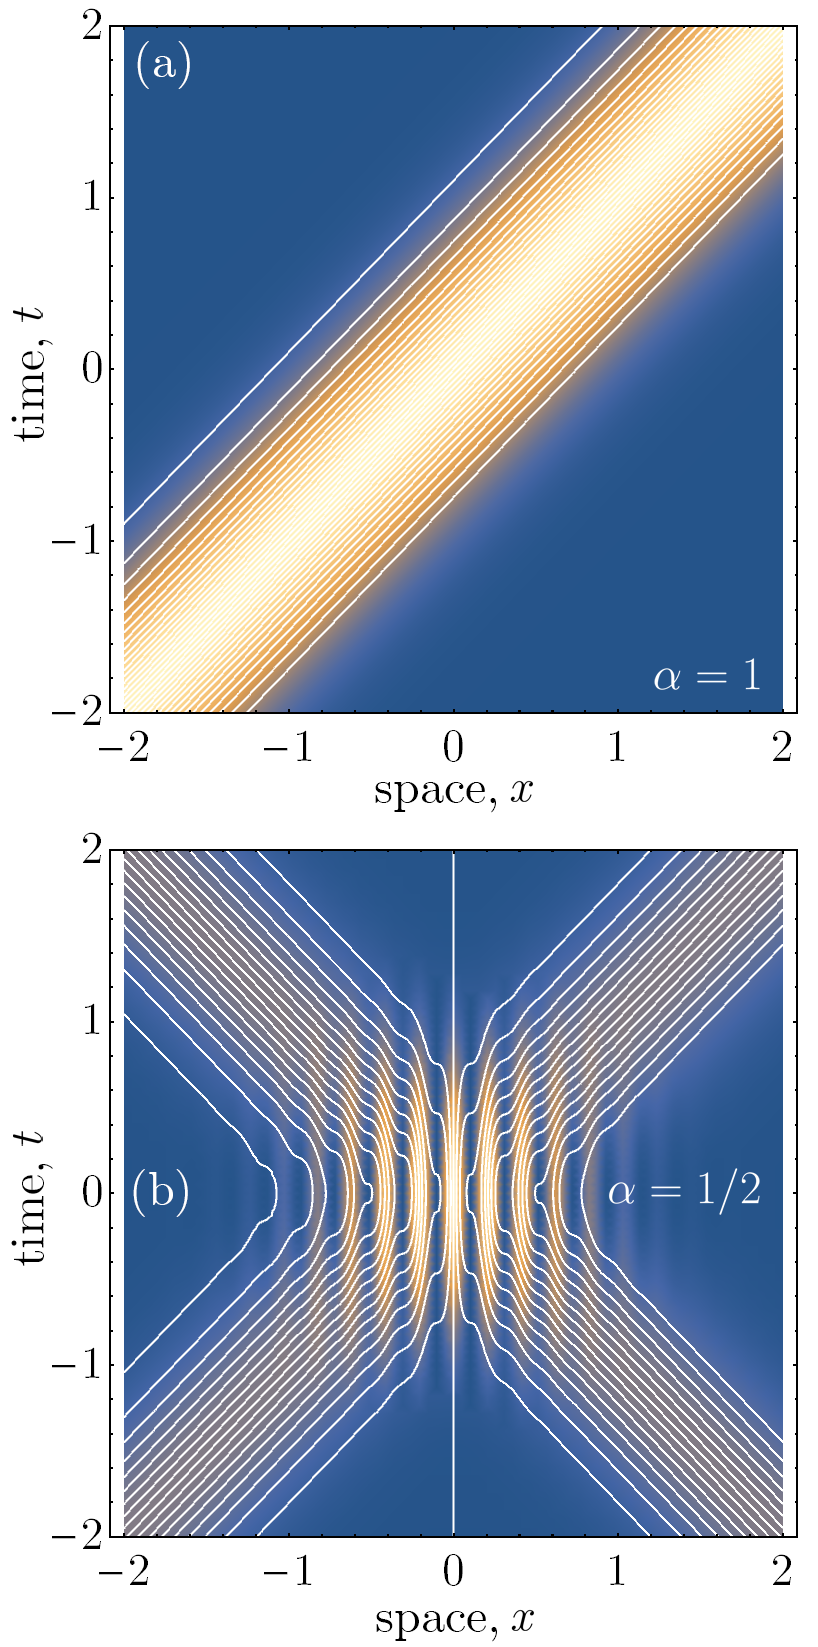
\includegraphics[width=0.8\linewidth]{Fig2trajectoriessimplified.png}
    \caption{Plots of the Bohmian trajectories with $k_0/\sigma = 15$. In the background of both plots is the quantum-mechanical prediction for the probability density of the particles, $\rho_{K}(x,t)$. In (a), the trajectories are completely right-moving and maintain a Gaussian distribution, according to the initial conditions that we have chosen to match the wavefunction density. In (b), we have considered the superposition case, wherein the photon follows a path which matches the interference pattern predicted by $\rho_K(x,t)$. }
    \label{fig:trajectories1}
\end{figure}

Before analysing the particle trajectories, it must be noted that Eq.\ (\ref{eq14}) is not positive definite, and thus generally cannot be interpreted as a probability density. Regions of negative density emerge when the last term of $\mathcal{T}_0$ becomes non-negligible. However since we focus our analysis on the optical regime where $k_0 \gg \sigma$, the magnitude of this term is small compared with the first, so that the density remains positive definite and can be interpreted as a true probability density. If one naively takes the density to be the modulus square of the wavefuncion, $| \psi(x,t)|^2$, one obtains Eq.\ (\ref{eq14}) without the final term in $\mathcal{T}_0$. 

In Fig.\ \ref{fig:trajectories1}, we have plotted the Bohmian trajectories for the particles in the head-on collision scenario for different weightings of the superposition parameter $\alpha$. The trajectories for different initial conditions (spaced in proportion to the wavepacket density) are shown in white, superimposed on top of the Klein-Gordon density. In Fig.\ \ref{fig:trajectories1}(a), the particles are moving solely in the right-moving direction. As expected for relativistic massless particles, the trajectories maintain a Gaussian profile without dispersion. Importantly, the density of trajectories corresponds exactly with the Klein-Gordon probability density, and this matching condition holds for all time. This is an essential consistency requirement of Bohmian mechanics, and the continuity equation plays a crucial role in ensuring this condition. Likewise in the equal superposition case, the density of trajectories matches exactly with the interference pattern predicted by $\rho_K(x,t)$. In regions of constructive interference the trajectories bunch up, while the opposite occurs for regions of destructive interference. Notably, some of the trajectories become superluminal in regions of destructive interference. 

\begin{figure}[h]
    \centering
    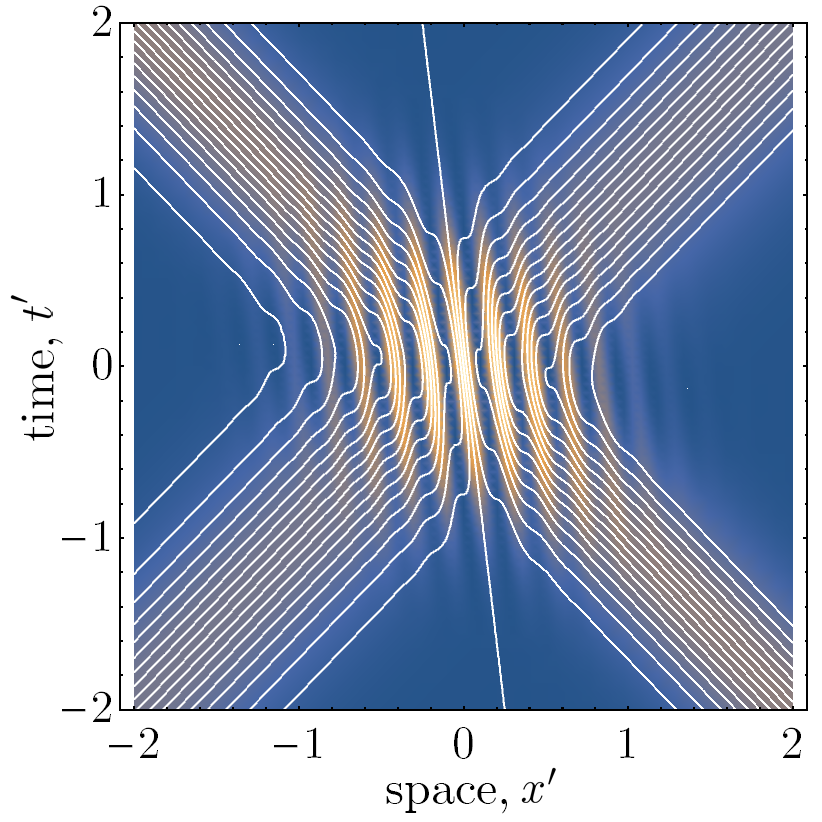
\includegraphics[width=0.8\linewidth]{Fig6boostedsimplified.png}
    \caption{Plot of the Bohmian trajectories with respect to the boosted coordinates of an observer who is moving at $v = 0.125$ with respect to the lab frame. We have used the parameters $k_0/\sigma  = 15$ as in Fig.\ \ref{fig:trajectories1}. }
    \label{fig:trajectoriesboost1}
\end{figure}
In Fig.\ \ref{fig:trajectoriesboost1}, we have plotted the Bohmian trajectories in the boosted coordinates of a moving observer. The regions of interference are now tilted with respect to these coordinates, since the observer is moving past the apparatus at a relativistic velocity. Due to the invariance of the continuity equation under boosts, the density of trajectories is conserved, matching the quantum-mechanical prediction.


\subsubsection{Relativistic grazing regime} 
We can also consider the general case with energy dispersion $E(k) = \sqrt{k^2 + k_z^2}$. If $k_z$ is constant and small but non-zero, this represents a grazing collision regime shown in Fig.\ \ref{fig:setup}(b). Since there is no simple expression in terms of elementray functions for the wavefunction integrals, we utilise a numerical analysis for this case. 
\begin{figure}[h]
    \centering
    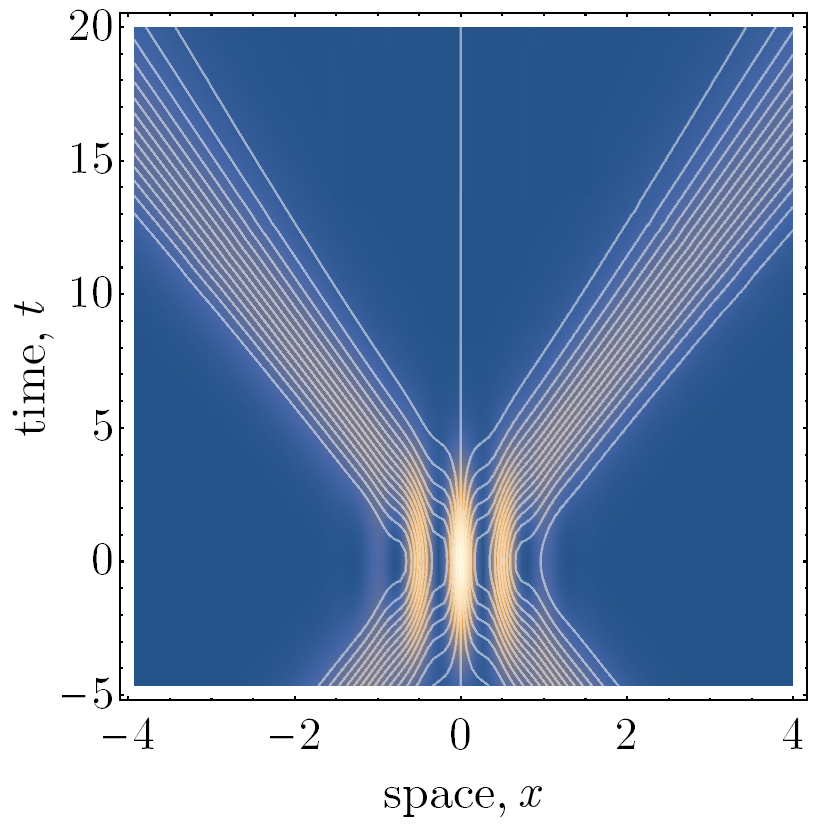
\includegraphics[width=0.8\linewidth]{Fig4subrelativistic.png}
    \caption{Bohmian trajectories in for a generic relativistic dispersion with $k_0/\sigma = 6$, $k_z/\sigma = 24$ and $\alpha = 1/2$. The effect of $k_z$ is to introduce some dispersion in the trajectory density as the particles propagate in time. }
    \label{fig:subrelativistic}
\end{figure}
Figure \ref{fig:subrelativistic} displays the Bohmian trajectories in the grazing relativistic regime. A notable feature is the dispersion of the trajectories as they propagate in time. This is due to the inclusion of the nonzero effective mass term $k_z$ in the particle energy. 


\subsubsection{Paraxial limit}
To obtain the nonrelativistic limit of our velocity equation, we consider the regime $k_z \gg k$, so that the total energy takes the form $E(k) \simeq k_z + k^2/2k_z$. As in the relativistic grazing regime, $k_z$ can be interpreted as a mass-like term. The velocity equation under this approximation becomes
\begin{align}\label{22paraxial}
    V(x,t) &= \frac{1}{2k_z}\frac{2\text{Im}\: \psi_S^\star(x,t)  \p^x \psi_S(x,t)}{|\psi_S(x,t)|^2}
\end{align}
where the wavefunction is explicitly 
\begin{align}
    \psi_S(x,t) &= \sqrt{\alpha}e^{-ik_zt} \int\D k \: e^{ikx -\frac{ik^2t}{2k_z}} f_R(k) \nonumber \\
    & + \sqrt{1 - \alpha}e^{-ik_zt } \int\D k \:e^{ikx - \frac{ik^2t}{2k_z}} f_L(k). 
\end{align}
We readily identify the numerator and denominator of Eq.\ (\ref{22paraxial}) with the nonrelativistic versions of the conserved current and density, 
\begin{align}
    V(x,t) &= \frac{j_S(x,t)}{\rho_S(x,t)} .
\end{align}
Of course, these quantities do not transform relativistically under Lorentz boosts, however they do obey Galilean invariance as expected. 
Notably, Eq.\ (\ref{22paraxial}) yields the same result as that derived by Wiseman who used the following definition for the velocity in the nonrelativistic, paraxial limit \cite{Wiseman_2007}:
\begin{align}\label{wiseman}
    V(x,t) &= \lim_{\delta t \to 0 } \frac{1}{\delta t} \left[ x - \prescript{}{\langle x | }{\langle \hat{x}_w \rangle}_{|\psi(t) \rangle} \right] .
\end{align}
\begin{figure}[h]
    \centering
    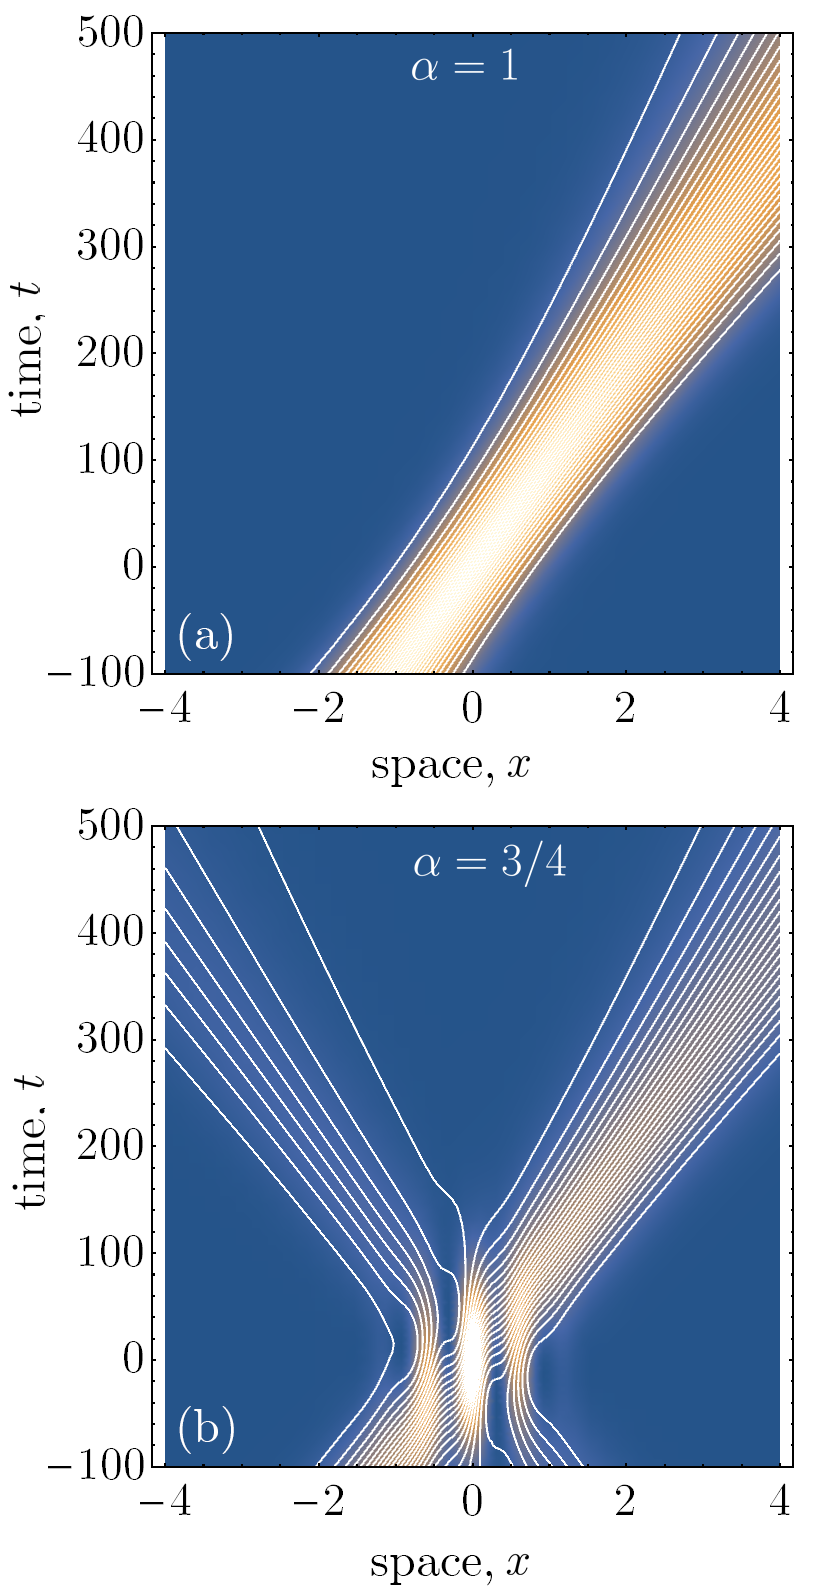
\includegraphics[width=0.8\linewidth]{Fig3paraxialtrajectoriesb.png}
    \caption{Plots of the Bohmian trajectories with $k_0/\sigma = 5$, $k_z/\sigma = 500$. As in the relativistic grazing limit, the particles exhibit dispersion as they propagate in time. Notably, this occurs on a much larger timescale as compared with the relativistic cases.}
    \label{fig:paraxial}
\end{figure}
Wiseman's approach in obtaining Eq.\ (\ref{wiseman}) was to perform a weak measurement of the particle position at time $t$, followed by a strong measurement of the position a short time $\delta t$ later. The velocity is obtained by calculating the rate of change of position over this small time interval, $\delta t$. When extending this equation to relativistic particles, it ultimately fails because it tacitly assumes a preferred reference frame (i.e.\ the lab frame). This can be seen in the introduction of the Lorentz noninvariant parameter $\delta t$ in the evolution between the weak and strong measurements. If the relativistic limit $E(k) \simeq |k|$ is naively applied to Eq.\ (\ref{wiseman}), it can be shown that the continuity equation is not satisfied in general. 

Nevertheless, Eq.\ (\ref{22paraxial}) and (\ref{wiseman}) are valid expressions for the Bohmian velocity of nonrelativistic particles. In Fig.\ \ref{fig:paraxial}, we have plotted these trajectories in the paraxial limit. Like the relativistic grazing scenario, the particles exhibit dispersion as they propagate in time. The slow-moving particle velocities cause the regions of interference to stretch out in time, comparing the timescales of Fig.\ \ref{fig:trajectories1} and Fig.\ \ref{fig:paraxial}. 


\subsection{The photon metric}
A key concept introduced in Bohm's theory is the quantum potential, $Q(x,t)$, which appears as an additional term in the so-called `quantum Hamilton-Jacobi' equation obtained from the Schr\"odinger equation \cite{bohm2006undivided}. In the paraxial limit for our single-photon system, the quantum potential takes the form
\begin{align}\label{potential}
    Q(x,t) &= - \frac{\hslash^2}{2k_z} \frac{\nabla^2 R(x,t)}{R(x,t)} ,
\end{align}
where $R^2(x,t) = | \psi(x,t) |^2$. Using Eq.\ (\ref{potential}), one can obtain the quantum analogue of a classical force, using the standard definition $F_Q(x,t) = - \nabla Q(x,t)$, and this ultimately governs the dynamics of the particle. Evidently, the wavefunction plays a crucial role in determining $Q(x,t)$. When extending Bohmian mechanics to relativistic regimes as we have done here, the `quantum force' obtained from the quantum potential may now be interpreted as being generated by a quantum spacetime metric. In this way, $\psi(x,t)$ still plays a role in governing the effective dynamics of the particle, but now by defining the shortest path through the spacetime in the paradigm of general relativity. 

The problem is that the dynamics generated by such a metric must allow for trajectories that have both spacelike and timelike tangents. A candidate for the kinds of head-on particle trajectories observed in Fig.\ \ref{fig:trajectories1} and \ref{fig:trajectoriesboost1} is the Alcubierre metric, given by 
\begin{align}\label{alcubierre}
    \D s^2 &= - (1 - v_s^2) \D t^2 - 2 v_s \D x \D t + \D x^2 
\end{align}
where we have suppressed the $\D z$ component for simplicity. Equation (\ref{alcubierre}) was proposed by Alcubierre in \cite{Alcubierre_1994} as a so-called warp drive solution to Einstein's field equations. In such a spacetime, particles can achieve superluminal velocities through a local expansion of spacetime behind them and a simultaneous contraction of the spacetime in front of them. As is the case with other non-hyperbolic metrics like wormholes
\cite{einsteinPhysRev.48.73,morrisdoi:10.1119/1.15620}, exotic matter (i.e.\ negative energy density \cite{fordPhysRevD.55.2082}) is required to produce such effects. Nevertheless, Eq.\ (\ref{alcubierre}) is a consistent solution within the framework of general relativity, and by defining
\begin{align}
    v_s &= \left( \left| \frac{j_{K}(x,t)}{\rho_{K}(x,t)} \right| - 1 \right) \text{sgn} \left( \frac{j_{K}(x,t)}{\rho_{K}(x,t)} \right) 
\end{align}
where $\text{sgn}(x)$ represents the function giving $+1$ on positive values and $-1$ on non-positive values of $x$, the speed of light according to a faraway observer in an asymptotically flat spacetime region is given by
\begin{align}
    c &= v_s + \text{sgn}\left(\frac{j_K(x,t)}{\rho_K(x,t)} \right) = \frac{j_K(x,t)}{\rho_K(x,t)} .
\end{align}
This is exactly the prediction of our proposed relativistic Bohmian theory, wherein the coordinate velocity of the particle can exceed the speed of light (i.e.\ in regions of destructive interference), but also equal zero; that is, when the photon stops and changes directions. Of course such behaviour is permissible within the paradigm of general relativity, which only requires that light always travels at the speed of light locally.

\section{Discussion}
In this article, we have extended the theory of single-particle Bohmian mechanics to include particles with relativistic energies, showing that such a description is consistent with Lorentz invariance and a modification to Wiseman's weak measurement formalism. This represents an important step in testing the limits of the Bohmian interpretation, which to date has been believed to break down in relativistic regimes.

As emphasised throughout this work, we have employed an optical approximation in our analysis, wherein the frequency of the incoming wavepackets is much larger than their variance, $k_0 \gg \sigma$. In this regime, the Klein-Gordon density remains strictly positive, allowing for its interpretation as a \textit{probability} density. However it is well-known that the $\rho_K(x,t)$ can become negative in certain regimes; in our system, this occurs when the optical limit is no longer satisfied, $k_0 \sim \sigma$. In this limit the second term of Eq.\ (\ref{21constant}) is no longer negligible, and in the regions previously associated with destructive interference of the wavefunction, the density can become negative. 

As noted previously, the matching condition between the density of Bohmian trajectories and the density of the guiding wave holds for all time, and this is true even in regions of negative density. In these regions, the tangent vector to the trajectory becomes negative, yielding particle trajectories which travel backwards in time. The negative density of these backward-in-time trajectories matches the regions of `negativity' in the wavefunction density, demonstrating the mathematical consistency of our theory in these regimes. Notably, it is well-known that the weak values of positive operators can be negative \cite{puseyPhysRevLett.113.200401,Hosoya_2010,sokolovskiPhysRevA.76.042125,johansenPhysRevA.70.052115,aharonovPhysRevA.72.052111}. However, a consistent physical interpretation of these trajectories likely requires an extension of our theory to a full field-theoretic description of the Bohmian mechanics that can handle multi-particle states. For example, one would expect that a more complete measurement model is needed, particularly one which is valid outside the optics limit we have considered here. By leaving the optical limit, one enters a subcycle regime (i.e.\ measurements occurring at timescales shorter than a single wavelength of light), wherein effects such as particle production emerge, a description requiring a full quantum field theory \cite{Riek_2017}. The mathematical consistency of our single-particle relativistic theory may give some guidance in such an endeavour. 

\begin{figure}[h]
    \centering
    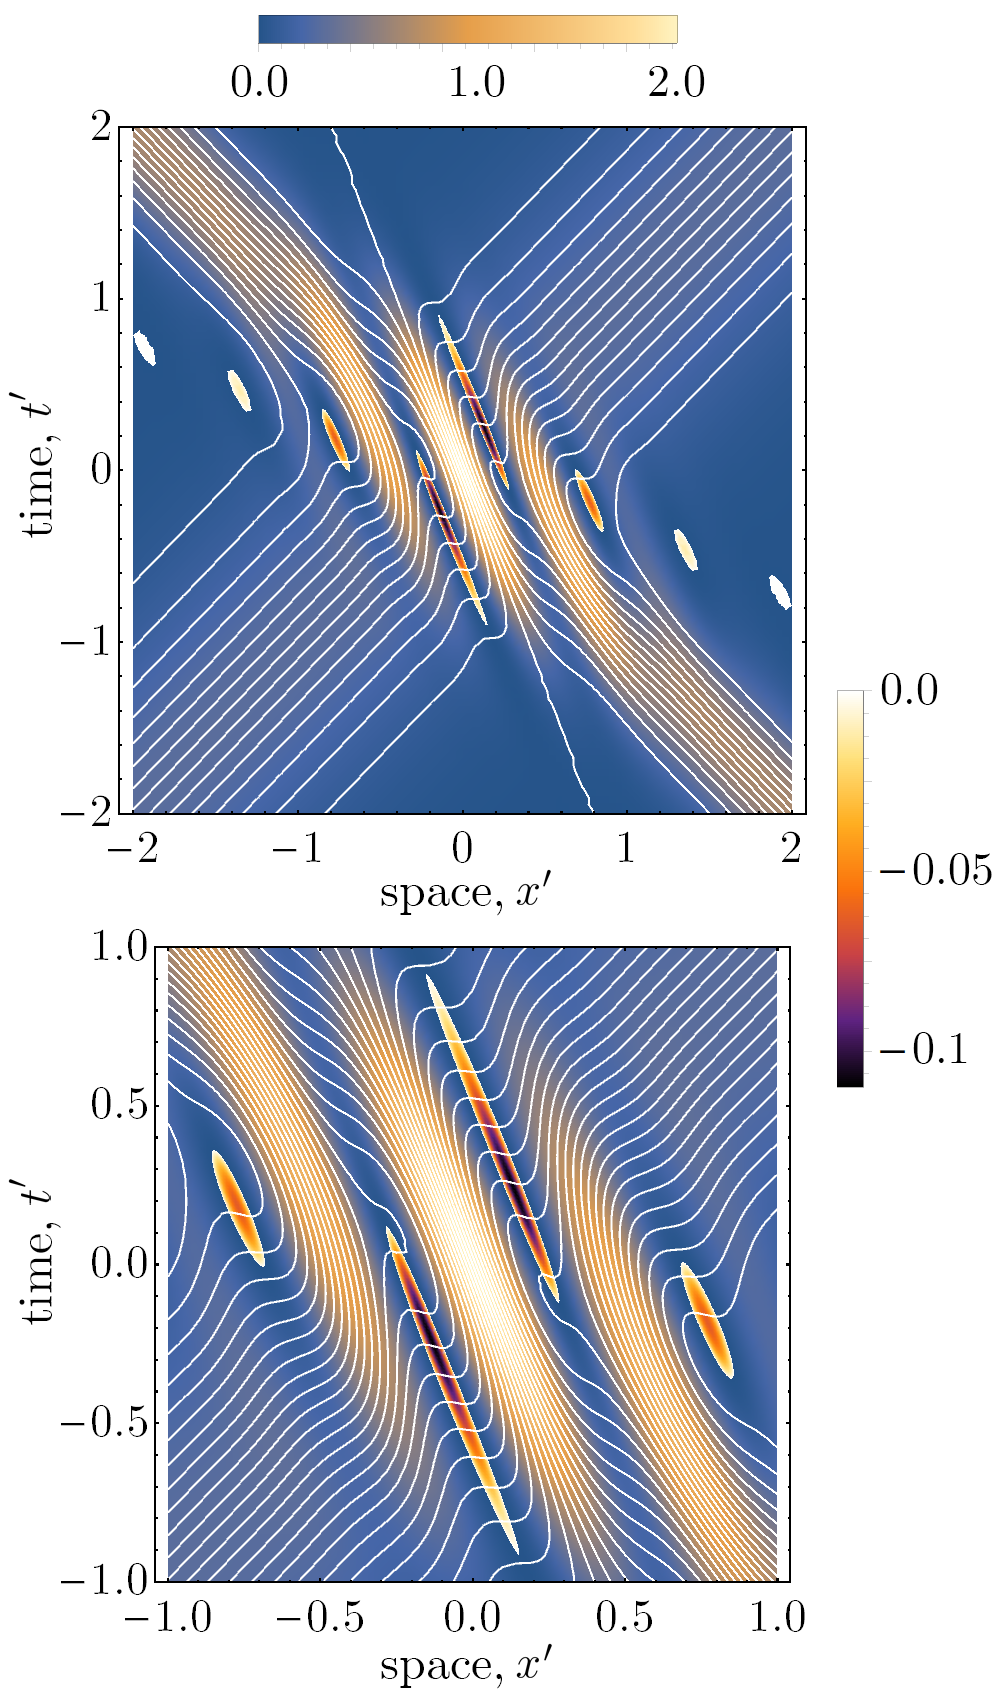
\includegraphics[width=0.925\linewidth]{Fig5negative.png}
    \caption{Bohmian trajectories in the head on limit, viewed from a boosted reference frame with $v = 0.4$, $k_0/\sigma = 6$ and $\alpha = 1/2$. The trajectories are superimposed over the corresponding Klein-Gordon density, where the respective legends show the magnitude of the positive and negative density regions. The lower panel shows a zoomed in view of the trajectories. }
    \label{fig:negative}
\end{figure}

The existence of backward-in-time Bohmian trajectories and hence negative densities is most clearly demonstrated by considering the particle trajectories according to observers in rapidly boosted reference frames, Fig.\ \ref{fig:negative}. When the Klein-Gordon density in the boosted frame equals zero,
\begin{align}
    0 &= \gamma ( \rho(x,t) - vj(x,t) ) ,
\end{align}
the particle velocity according to an observer in this frame, 
\begin{align}
    V'(x,t) &= \frac{V(x,t) - v}{1 - v V(x,t)} ,
\end{align}
diverges. It can be seen that this property is inevitable for superluminal particle velocities satisfying the velocity addition rule. The divergence of the velocity occurs for pairs of spacetime points; as shown in Fig.\ \ref{fig:negative}, the particle `enters' the region of negative density at infinite velocity, travels backwards in time for some distance, before `exiting' this region at another point with infinite velocity. As stated previously, modelling detection of these negative density regions requires a more complete measurement model; one understands that the timescales required to observe the backward-in-time trajectories enter a regime where subcycle effects become important. 

As mentioned, Bohmian trajectories have been observed experimentally for photons which are transversely slow (i.e.\ the paraxial limit) \cite{kocsis2011observing, mahler2016experimental}. In those experiments, the velocity field of the photons was reconstructed by performing weak measurements of momentum, postselected at a particular spacetime position. This is complementary to Wiseman's definition, Eq.\ (\ref{wiseman}). To perform the weak measurements, the photon polarisation was utilised as a pointer which coupled to the momentum \cite{kocsis2011observing}. In our model, constructing the velocity field of the transversely fast photons also requires weak measurements of momentum, so the above mentioned approach may be applied analogously. Of course, since the transverse velocities are now relativistic, these measurements may be technically challenging but nevertheless possible in principle. Meanwhile, weak measurements of the particle energy in the case of photons essentially requires a measurement of its frequency. This has been achieved for example by weakly perturbing the path of a frequency-modulated beam using an adjustable prism, from which weak measurements of the induced frequency shift can be inferred \cite{starlingPhysRevA.82.063822,zhouPhysRevA.95.042121,dresselRevModPhys.86.307}. 

The approach we have introduced in this article motivates numerous pathways for further research. A natural extension of our model would be to study a system with multiple particles, for which the nonlocality of Bohmian mechanics in the relativistic regime may be properly understood. As in the single-particle case, Bohmian-mechanical models for multiple particle scenarios have been developed in the nonrelativistic regime. Braverman and Simon \cite{bravermanPhysRevLett.110.060406} first proposed a model for path-entangled photons in a double-slit experiment, wherein the velocity of the photon entering the apparatus depends on the value of a phase shift applied to the second photon in a spacelike separated region. This was then implemented in the experiment by Mahler et.\ al.\ \cite{mahler2016experimental}, giving strong empirical verification of the nature of nonlocal influences in the Bohmian paradigm. How such entanglement manifests in the relativistic domain remains an interesting question. Another important question to answer is the consistency of our model outside the self-imposed optical limit. We studied this regime to obtain physically interpretable results, in line with the constraints of our single-particle theory. The possibility of constructing a full Bohmian quantum field theory, allowing for the study of particle production effects and subcycle optical regimes, remains a tantalising prospect.   

\section{Methods}
\subsection{Derivation of the relativistic velocity equation}
Recall our proposed form for the weak value definition of the velocity equation:
\begin{align}
    V(x,t) &= \frac{\prescript{}{\langle x |}{\langle \hat{k}_w \rangle_{|\psi(t)\rangle} }}{\prescript{}{\langle x | }{\langle \hat{H}_w \rangle_{|\psi(t) \rangle} }} = \frac{\text{Re} \langle x | \hat{k}  | \psi(t)\rangle}{\text{Re} \langle x | \hat{H} | \psi(t)\rangle} .
\end{align}
We calculate the numerator and denominator individually.  To this end, we need to give values for the $\bra{x}\hat{A}\ket{\psi(t)}$ expressions in the theory we use.  With $\hat{A} = I$ the identity operator, the identification is trivially $\braket{x|\psi(t)}=\psi(x,t)$, the one particle Klein-Gordon field solution.  The momentum operator $\hat{k}$ is formed from the generator of displacements in position.  So by the standard definition we can write
\[
\bra{x}\hat{k}\ket{\psi(t)} = - i \p_x \psi(x,t) = - i \p^x \psi(x,t),
\]
where the Minkowski metric has been used to raise the derivative index. Similarly, the generator of temporal displacements in the field are associated with the Hamiltonian operator and hence
\[
\bra{x}\hat{H}\ket{\psi(t)} = i \p_t \psi(x,t)= - i \p^t \psi(x,t).
\]
The weak-value expressions can be evaluated using these identifications for momentum
\begin{align}
    \wv{\bra{x}}{\hat{k}}{\ket{\psi(t)}} 
    &= \text{Re} \frac{\bra{x} \hat{k} \ket{\psi(t)}}{\braket{x | \psi(t)}} , \nonumber \\
    &= \text{Re} \frac{\braket{\psi(t)| x}}{|\braket{x | \psi(t)}|^2} \bra{x} \hat{k} \ket{\psi(t)} \nonumber , \\
    &= \text{Re} \frac{(-i) \psi^\star(x,t) \p^x \psi(x,t)}{| \psi(x,t) |^2 },
\end{align}
and energy
\begin{align}
    \wv{\bra{x}}{\hat{H}}{\ket{\psi(t)}} 
    &= \text{Re} \frac{\bra{x} \hat{H} \ket{\psi(t)}}{\braket{x | \psi(t)}} , \nonumber \\
    &= \text{Re} \frac{\braket{\psi(t)| x}}{|\braket{x | \psi(t)}|^2} \bra{x} \hat{H} \ket{\psi(t)} \nonumber,  \\
    &= \text{Re} \frac{(-i) \psi^\star(x,t) \p^t \psi(x,t)}{| \psi(x,t) |^2 }.
\end{align}
Dividing the two weak values yields,
\begin{align}
    V(x,t) &= \frac{\text{Re}(-i)\psi^\star(x,t) \p^x \psi(x,t)  }{\text{Re} \: (-i) \psi^\star(x,t) \p^t \psi(x,t)}, \nonumber \\ 
    &= \frac{2 \text{Im} \: \psi^\star(x,t) \p^x \psi(x,t)}{2 \text{Im} \: \psi^\star(x,t) \p^t  \psi(x,t)}.
\end{align}
The numerator and denominator are exactly the Klein-Gordon conserved probability current and density, as shown in the main text. 

\subsection{Position space wavefunction in the head-on limit}
In the head-on limit, the particle energy can be approximated as $E(k) = |k|$. The position space wavefunction is given by 
\begin{align}
    \psi_K(x,t) &= \sqrt{\alpha} \int \D k \: f_R(k) e^{-i|k|t + i kx } \non \\
    & + \sqrt{1 - \alpha} \int \D k \:f_L(k) e^{-i|k|t + i kx }.
\end{align}
We make the assumption that the wavepackets $f_L(k)$ and $f_R(k)$ are only non-negligible in the regions $k<0$ and $k>0$ respectively. This is to remain consistent with the quantum-optical regime that we are restricting our analysis to. One can write
\begin{align}\label{37}
    \psi_K(x,t) &\simeq \sqrt{\alpha} \int_0^\infty \D k \:f_R(k) e^{-i|k|t + i kx } \non \\
    & + \sqrt{1 - \alpha } \int_{-\infty }^0 \D k \: f_L(k) e^{-i|k|t + i kx } \\
    \intertext{Using the strictly positive domains of the integral bounds to eliminate the absolute value signs in the exponents yields,}
    \psi_K(x,t) &= \sqrt{\alpha} \int_0^\infty\D k \:f_R(k) e^{-ik(t -x ) } \non \\
    & + \sqrt{1 - \alpha} \int_0^\infty\D k \: f_L(-k) e^{-ik(t + x) }.
    \intertext{Using the assumptions on $f_L(k)$ and $f_R(k)$, we can then extend the bounds on the integrals without significant error:}\label{44}
    \psi_K(x,t) &= \sqrt{\alpha} \infint \D k \:f_R(k) e^{-ik(t-x)} \non \\
    & + \sqrt{1 -\alpha} \infint \D k \:f_L(-k) e^{-ik(t +x) }. 
    \intertext{Equation (\ref{44}) can be evaluated analytically. In the simple case where $k_{0R} = k_{0L} \equiv k_0$ and $\sigma_R = \sigma_L \equiv \sigma$, the wavepacket normalisation constants are simply $(2\pi \sigma)^{-1/4}$, giving}\label{eq45psi}
    \psi_K(x,t) &= \mathcal{J}_0 \bigg[ \sqrt{\alpha} \exp \Big[ - (t-x) \mathcal{V}_R \Big] \non \\
    & + \sqrt{1 - \alpha}  \exp \Big[ - (t+ x)  \mathcal{V}_L \Big]   \bigg] 
\end{align}
where $\mathcal{J}_0 = (2\sigma^2/\pi)^{1/4}$ and
\begin{align}
    \mathcal{V}_R &= ik_0 + (t-x)\sigma^2 \vphantom{\frac{1}{2}}, \\
    \mathcal{V}_L &= ik_0 + (t+x)\sigma^2 . 
\end{align}
Inserting Eq.\ (\ref{eq45psi}) into the expressions for the relativistic Klein-Gordon probability current and density,
\begin{align}
    j_K(x,t) &= 2 \text{Im} \:\psi^\star(x,t) \p^x \psi(x,t)  \vphantom{\frac{1}{2}} , \\
    \rho_K(x,t) &= 2 \text{Im} \: \psi^\star(x,t) \p^t \psi(x,t) ,
\end{align}
then we straightforwardly obtain Eq.\ (\ref{jkeq18}) and Eq.\ (\ref{eq14}) stated in the main text. 


\subsection{Paraxial limit of the relativistic velocity equation}
We can obtain the nonrelativistic velocity equation by taking the paraxial limit of our relativistic velocity equation. Firstly, in the paraxial limit, the energy of the photon is $E(k) \simeq k_z + k^2/2k_z$ for $k \ll k_z$. The wavefunction can be written as
\begin{align}
    \psi_S(x,t) &= \int\D k \: e^{ikx } e^{-ik_z t - \frac{ik^2t}{2k_z}} f(k) 
\end{align}
where $f(k) = \sqrt{\alpha} f_R(k) + \sqrt{1 - \alpha}f_L(k)$ using $f_L$ and $f_R$ defined in Eqs.~(\ref{f_right}) and~(\ref{f_left}).  We are also assuming that $f(k)$ is not supported outside of the $k \ll k_z$ approximation. Inserting $\psi_S(x,t)$ into the Klein-Gordon expression for the probability density will give the density appropriate for these approximations, which can be manipulated to give
\begin{align}
    \rho_K(x,t) &= 2 \text{Im}
    \int\D k \int\D k' f^\star(k) f(k') \nonumber \vphantom{\int} \\
    & \quad \exp \Big[ -ik^\prime x \Big] \exp \Big[ ik_zt + \frac{it{k^\prime}^2}{2k_z} \Big] \non \vphantom{\int} \\
    & \quad  \left(-\frac{\partial}{\partial t}\right)
    \left(\exp \Big[ ik'x \Big]
    \exp \Big[ -ik_zt - \frac{itk'^2}{2k_z} \Big] \right)
    \nonumber , \\
    &= 2 \text{Im}  
    \int\D k \int\D k' f^\star(k) f(k') 
    \left( i k_z + \frac{ik'^2}{2k_z} \right) \nonumber \\
    & \quad \exp \Big[ -i(k-k')x \Big]
    \exp \Big[ \frac{it}{2k_z}({k}^2 - k'^2) \Big]
    , \nonumber \vphantom{\int}  \\
    \intertext{Recognising that $k'^2$ can be expressed in differential operator form as $- \p^2/\p x^2$ and that the double integral expression is simply $\psi_S^\star(x,t) \psi_S(x,t)$, we obtain the simplified form}
    \rho_K(x,t) &= 2 \text{Im} \Big[ 
    ik_z |\psi_S(x,t)|^2 -\frac{i}{2k_z} \psi_S^*(x,t) \frac{\partial^2 \psi_S(x,t) }{\partial^2 x}
    \Big] , \nonumber \vphantom{\int}  \\
    &\simeq  2 k_z | \psi_S(x,t) |^2 = 2k_z \rho_S(x,t),
    \vphantom{\int} 
\end{align}
where in the final line the approximation used is that the double spatial derivative of $\psi_S$ is negligible compared to $k_z^2$.
The velocity equation in the paraxial limit thus becomes
\begin{align}
    V(x,t) &= \frac{1}{2k_z} \frac{2\text{Im} \: \psi_S^\star(x,t) \p^x \psi_S (x,t) }{| \psi_S(x,t) |^2}.
\end{align}
This is simply the nonrelativistic definition of the velocity, expressed in terms of the Schr\"odinger probability current and density. This is exactly the form obtained using Wiseman's nonrelativistic weak value formula in \cite{Wiseman_2007}.


\subsection{Analytic expression for the Bohmian velocity in the paraxial limit}
Let us derive the analytic form of the paraxial limit velocity. Again, applying the optical approximation used in Eq.\ (\ref{37}), for an initial superposition of left- and right-moving wavepacket the wavefunction in the paraxial limit is given by 
\begin{align}
    \psi_S(x,t) &= \sqrt{\alpha} e^{-i k_z t } \int\D k \:e^{ikx- \frac{ik^2 t}{2k_z}} f_R(k) \non \\
    & + \sqrt{1 - \alpha} e^{-ik_z t} \int\D k \:e^{-ikx - \frac{ik^2t}{2k_z}} f_L(-k)  .
\end{align}
The integrals can be evaluated analytically. The components of the probability current can be split into left- and right-moving parts, and an interference term which mixes these components. These are given by 
\begin{align} 
    j_L(x,t) &= - \mathcal{C}_0 \exp \left[ - \frac{2(k_0t - k_zx)^2 \sigma^2}{k_z^2 + 4t^2 \sigma^4} \right], \nonumber \\
    j_R(x,t) &= \mathcal{D}_0 \exp \left[ -\frac{2(k_0t + k_zx)^2}{k_z^2 + 4t^2\sigma^4} \right], \nonumber \\
    j_I(x,t) &= \mathcal{L}_0 \exp \left[ - \frac{2(ik_0k_z^2x+k_{tx}\sigma^2)}{k_z^2 + 4t^2\sigma^4} \right] ,
\end{align}
where we have defined $k_{tx} = k_0^2t^2+k_z^2x^2$ and
\begin{align}
    \mathcal{C}_0 &= \mathcal{M}_0 (k_0 k_z + 4tx\sigma^4) \vphantom{\sqrt{\frac{2}{\pi}}}, \nonumber \\
    \mathcal{D}_0 &= \mathcal{M}_0 (k_0 k_z - 4tx \sigma^4) \vphantom{\sqrt{\frac{2}{\pi}}} , \nonumber \\
    \mathcal{M}_0 &= \sqrt{\frac{2}{\pi}} \frac{k_z\sigma}{2(k_z^2 + 4t^2\sigma^4)^{3/2}}
    \vphantom{\sqrt{\frac{2}{\pi}}} ,
\end{align} 
and
\begin{align}
    \mathcal{L}_0 &= 4 \sigma t \mathcal{M}_0 \bigg[ 2x \sigma^2 \left( 1 + \exp \left[ \frac{4ik_0k_z^2x}{k_z^2 + 4t^2\sigma^4} \right] \right) \non \\
    & + ik_0 \left( 1 - \exp \left[ \frac{4ik_0 k_z^2x}{k_z^2 + 4t^2\sigma^4} \right] \right) \bigg] .
\end{align}
Similarly, the density can likewise be decomposed into left- and right-moving parts, and an interference term. These are,
\begin{align}
    \rho_L(x,t) &= \mathcal{K}_0 \exp \left[ -\frac{2(k_0t + k_zx)^2 \sigma^2}{k_z^2 + 4t^2\sigma^4} \right] , \nonumber  \\
    \rho_R (x,t) &= \mathcal{K}_0  \exp \left[ - \frac{2(k_0t - k_zx)^2\sigma^2}{k_z^2 + 4t^2\sigma^4} \right], \nonumber \\
    \rho_I (x,t) &= \mathcal{K}_e  \exp \left[ - \frac{2(ik_0k_z^2 x + k_{tx}\sigma^2)}{k_z^2 + 4t^2 \sigma^4} \right] ,
\end{align}
where we have defined 
\begin{align}
    \mathcal{K}_0 &= \sqrt{\frac{2}{\pi}} \frac{k_z\sigma}{\sqrt{4t^2\sigma^4 + k_z^2}}  , \nonumber \\
    \mathcal{K}_e &= \mathcal{K}_0 \left( 1 + \exp \left[ \frac{4ik_0 k_z^2x}{k_z^2 + 4t^2\sigma^4} \right] \right) .
\end{align}
These expressions for the probability and current density are used to construct the trajectories shown in Fig.\ \ref{fig:paraxial}. 
\\\\

\acknowledgements
This research was supported by the Australian Research Council Centre of Excellence for Quantum Computation and Communication Technology (Project
No. CE170100012).

\bibliography{main} 



\end{document}


